%-%-%-%-%-%-%-%-%-%-%-%-%-%-%-%-%-%-%-%-%-%-%-%-%-%-%-%-%-%-%-%-%-%-%-%-%-%-%
%%% MAIN DOCUMENT %%%

%-%-%-%-%-%-%-%-%-%-%-%-%-%-%-%-%-%-%-%-%-%-%-%-%-%-%-%-%-%-%-%-%-%-%-%-%-%-%

\documentclass[12pt, oneside]{book}
\usepackage{xcolor}
\usepackage{minted}

% \usepackage[T1]{fontenc}

\usepackage{draculatheme}
\newcommand{\documentTheme}{draculafg}
\newcommand{\documentLogo}{../../images/small logo_white.png}
\newcommand{\documentBigLogo}{../../images/logo_white_text.png}
\usemintedstyle{dracula}

\usemintedstyle{dracula}

\setminted{
    linenos=true,
    numbersep=5pt,
    frame=lines,
    framesep=2mm,
    breaklines=true
}

% \newcommand{\documentBigLogo}{../../images/Hendrix Logo.png}
% \newcommand{\documentLogo}{../../images/small logo.png}
% \newcommand{\documentTheme}{black}

%%% AESTHETICS %%%
%-%-%-%-%-%-%-%-%-%-%-%-%-%-%-%-%-%-%-%-%-%-%-%-%-%-%-%-%-%-%-%-%-%-%-%-%-%-%


%%% Dimensions and Spacing %%%
\usepackage[margin=1in]{geometry}
\setlength{\parindent}{0pt}
\usepackage{setspace}
\usepackage{mathtools}
\usepackage{esint}
\usepackage{adjustbox}
\linespread{1}
\usepackage{listings}
\usepackage{tikz}
\usetikzlibrary{shapes,backgrounds,calc,patterns,positioning}
\usepgflibrary{shadings}
\usepackage{pgfkeys}
\usepackage{pdftexcmds}
\usepackage{shellesc}
\usepackage{algorithm, algorithmic, xspace}
%%% Define new colors %%%
\definecolor{orangehdx}{rgb}{0.96, 0.51, 0.16}

% Normal colors
\definecolor{xred}{HTML}{BD4242}
\definecolor{xblue}{HTML}{4268BD}
\definecolor{xgreen}{HTML}{52B256}
\definecolor{xpurple}{HTML}{7F52B2}
\definecolor{xorange}{HTML}{FD9337}
\definecolor{xdotted}{HTML}{999999}
\definecolor{xgray}{HTML}{777777}
\definecolor{xcyan}{HTML}{80F5DC}
\definecolor{xpink}{HTML}{F690EA}
\definecolor{xgrayblue}{HTML}{49B095}
\definecolor{xgraycyan}{HTML}{5AA1B9}

% Dark colors
\colorlet{xdarkred}{red!85!black}
\colorlet{xdarkblue}{xblue!85!black}
\colorlet{xdarkgreen}{xgreen!85!black}
\colorlet{xdarkpurple}{xpurple!85!black}
\colorlet{xdarkorange}{xorange!85!black}
\definecolor{xdarkcyan}{HTML}{008B8B}
\colorlet{xdarkgray}{xgray!85!black}

% Very dark colors
\colorlet{xverydarkblue}{xblue!50!black}

% Document-specific colors
\colorlet{normaltextcolor}{black}
\colorlet{figtextcolor}{xblue}

% Enumerated colors
\colorlet{xcol0}{black}
\colorlet{xcol1}{xred}
\colorlet{xcol2}{xblue}
\colorlet{xcol3}{xgreen}
\colorlet{xcol4}{xpurple}
\colorlet{xcol5}{xorange}
\colorlet{xcol6}{xcyan}
\colorlet{xcol7}{xpink!75!black}

% Blue-Purple (should just used colorbrewer...)
\definecolor{xrainbow0}{HTML}{e41a1c}
\definecolor{xrainbow1}{HTML}{a24057}
\definecolor{xrainbow2}{HTML}{606692}
\definecolor{xrainbow3}{HTML}{3a85a8}
\definecolor{xrainbow4}{HTML}{42977e}
\definecolor{xrainbow5}{HTML}{4aaa54}
\definecolor{xrainbow6}{HTML}{629363}
\definecolor{xrainbow7}{HTML}{7e6e85}
\definecolor{xrainbow8}{HTML}{9c509b}
\definecolor{xrainbow9}{HTML}{c4625d}
\definecolor{xrainbow10}{HTML}{eb751f}
\definecolor{xrainbow11}{HTML}{ff9709}

%------- %
% XHFILL %
%------- %



%%% Chapter Headings %%%

\newcommand{\gradientrule}{
    \begin{tikzpicture}
        \shade[left color=orangehdx, right color=black, middle color=gray] (0,0) rectangle (\linewidth,0.4pt);
    \end{tikzpicture}
}

\usepackage[Glenn]{fncychap}
\ChTitleVar{\bfseries\scshape\color{\documentTheme}} % Needed for Dracula theme
\ChNumVar{\large\selectfont\color{\documentTheme}} % Needed for Dracula theme
\ChNameVar{\large\color{\documentTheme}} % Needed for Dracula theme
\usepackage{xpatch}


\xpatchcmd\DOCH
{\mghrulefill}{\color{orangehdx}\mghrulefill}
{}{\PatchFailed}
\xpatchcmd\DOTI
{\mghrulefill}{\color{orangehdx}\mghrulefill}
{}{\PatchFailed}
\xpatchcmd\DOTIS
{\mghrulefill}{\color{orangehdx}\mghrulefill}
{}{\PatchFailed}



%% Change Chapter Heading Placement %%
\usepackage{etoolbox}
\makeatletter
\patchcmd{\@makechapterhead}{\vspace*{50\p@}}{\vspace*{-20\p@}}{}{}
\patchcmd{\@makeschapterhead}{\vspace*{50\p@}}{\vspace*{-20\p@}}{}{}
\patchcmd{\DOTI}{\vskip 80\p@}{\vskip 40\p@}{}{}
\patchcmd{\DOTIS}{\vskip 40\p@}{\vskip 0\p@}{}{}
\makeatother



\renewcommand{\thesection}{\thechapter.\arabic{section}} %% Chapter.Section Numbering


%%% listingS %%%
\usepackage{graphicx}  
% \numberwithin{listing}{section}
\usepackage{float}
\usepackage{caption}

%%% Hyperlinks %%%
\usepackage{hyperref}
\definecolor{horange}{HTML}{f58026}
\hypersetup{
	colorlinks=true,
	linkcolor=horange,
	filecolor=horange,      
	urlcolor=horange,
}

\newcommand{\assignmentname}{Homework 5: Chapters 5 \& 6}

%% Headers and Footers %%
\usepackage{fancyhdr} % This should be set AFTER setting up the page geometry
\pagestyle{fancy} % options: empty , plain , fancy
\fancyhead[R]{\textcolor{draculafg}{\assignmentname}}
\fancyhead[L]{\textcolor{draculafg}{Hendrix College}}
\fancyhead[C]{\includegraphics[height=.50cm]{\documentLogo}} % Use for Dracula
\usepackage{xpatch}
\xpretocmd\headrule{\color{orangehdx}}{}{\PatchFailed}
\setlength{\footskip}{0.5in}
\setlength{\headheight}{18.5764pt}


%%%%% Colored Boxes %%%%%
\usepackage{tcolorbox}
\tcbuselibrary{skins}
\tcbuselibrary{theorems}
% \tcbuselibrary{minted}
\newcounter{BoxCounter}
\usepackage{dingbat}

%-%-%-%-%-%-%-%-%-%-%-%-%-%-%-%-%-%-%-%-%-%-%-%-%-%-%-%-%-%-%-%-%-%-%-%-%-%-%

%% MATH PACKAGES, ENVIRONMENTS, COMMANDS %%
%-%-%-%-%-%-%-%-%-%-%-%-%-%-%-%-%-%-%-%-%-%-%-%-%-%-%-%-%-%-%-%-%-%-%-%-%-%-%
%You'll need your own packages, theorem types, and commands.

\usepackage{fix-cm}
\usepackage{amsmath,amsthm} 
\usepackage{array, makecell}
\usepackage{colortbl}
\newcommand{\thickvrule}{\vrule width 1pt}

\newcommand{\thickhrule}{\Xhline{1pt}}

\usepackage{mathtools}
\usepackage{amssymb}
\usepackage[framemethod=tikz]{mdframed}
\usepackage{mathrsfs}
\usepackage{changepage}
\usepackage{multicol}
\usepackage{slashed}
\usepackage{enumerate}
\usepackage{braket}
\usepackage{booktabs}
\usepackage{enumitem}
\usepackage{kantlipsum}  %This package lets us generate random text for example purposes.
\usepackage{pgfplots}


%%% Custom Commands %%%
% Natural Numbers 
\newcommand{\N}{\mathbb{N}}

% Whole Numbers
\newcommand{\W}{\mathbb{W}}

% Integers
\newcommand{\Z}{\mathbb{Z}}

% Rational Numbers
\newcommand{\Q}{\mathbb{Q}}

% Real Numbers
\newcommand{\R}{\mathbb{R}}

% Complex Numbers
\newcommand{\C}{\mathbb{C}}

\newcommand{\I}{\mathbb{I}}

\newcommand{\pfs}{\noindent\makebox[\linewidth]{\rule{\textwidth}{0.4pt}}\vspace{0.5cm}}

\newcommand{\mysqrt}[1]{%
	\mathpalette\foo{#1}%
}
\newcommand{\dmysqrt}[1]{%
	\mathpalette\foodisplay{#1}%
}

% !TeX spellcheck = off
\newcommand{\foo}[2]{%
	% #1: math style, #2: content
	\sbox0{$#1\sqrt{#2}$}% Measure the size of the standard sqrt in the current style
	\begin{tikzpicture}[baseline=(sqrt.base)]
		\node[inner sep=0, outer sep=0] (sqrt) {$#1\sqrt{#2}$}; % Use the current math style
		\draw([yshift=-0.045em]sqrt.north east) -- ++(0,-0.5ex); % Draw the tick
	\end{tikzpicture}%
}
% !TeX spellcheck = off
\newcommand{\foodisplay}[2]{%
	% #1: math style, #2: content
	\sbox0{$#1\sqrt{#2}$}% Measure the size of the standard sqrt in the current style
	\begin{tikzpicture}[baseline=(sqrt.base)]
		\node[inner sep=0, outer sep=0] (sqrt) {$\displaystyle\sqrt{#2}$}; % Force displaystyle
		\draw[line width=0.4pt] ([yshift=-0.044em]sqrt.north east) -- ++(0,-0.5ex); % Draw the tick
	\end{tikzpicture}%
}

\renewcommand{\theenumi}{\arabic{enumi}}
\renewcommand{\labelenumi}{\textbf{\theenumi}.}
\renewcommand{\theenumii}{\alph{enumii}}
\renewcommand{\labelenumii}{\textbf{\theenumii}.}

% \newcommand{}{\marginnote{
\includegraphics[width=2em]{caution.png}}}

\newmdenv[
	topline=false,
	bottomline=true,
	rightline=false,
	leftline=true,
	linewidth=1.5pt,
	linecolor=black, % default color, will be overridden in custom commands
	backgroundcolor=draculabg, % Needed for Dracula theme
	fontcolor=\documentTheme, % Needed for Dracula theme
	innertopmargin=0pt,
	innerbottommargin=5pt,
	innerrightmargin=10pt,
	innerleftmargin=10pt,
	leftmargin=0pt,
	rightmargin=0pt,
	skipabove=\topsep,
	skipbelow=\topsep,
]{customframedproof}

\newenvironment{proofpart}[2][black]{
    \begin{mdframed}[
        topline=false,
        bottomline=false,
        rightline=false,
        leftline=true,
        linewidth=1pt,
        linecolor=#1!40, % Custom color
        % innertopmargin=10pt,
        % innerbottommargin=10pt,
        innerleftmargin=10pt,
        innerrightmargin=10pt,
        leftmargin=0pt,
        rightmargin=0pt,
        % skipabove=\topsep,
        % skipbelow=\topsep%
    ]
    \noindent
    \begin{minipage}[t]{0.08\textwidth}%
        \textbf{#2}%
    \end{minipage}%
    \begin{minipage}[t]{0.90\textwidth}%
        \begin{adjustwidth}{0pt}{0pt}%
}{
    \end{adjustwidth}
    \end{minipage}
    \end{mdframed}
}

% Define a new environment 'proofscratch' for Proof and Scratch Paper
\newenvironment{proofscratch}[2]{%
    \begin{mdframed}[
        topline=false,
        bottomline=false,
        rightline=false,
        leftline=false,
        backgroundcolor=draculabg, % Background color for Dracula theme
        fontcolor=\documentTheme,       % Font color for Dracula theme
        innerleftmargin=-6pt,
        innertopmargin=0pt,
        leftmargin=0pt,
        rightmargin=0pt,
        skipabove=\topsep,
        skipbelow=\topsep,
    ]
    % % Begin TikZ picture for the vertical dotted line
    % \begin{tikzpicture}[overlay, remember picture]
    %     % Draw a vertical dotted line at approximately the center of the mdframed width
    %     \draw[dotted, thick] ([xshift=0.005\linewidth]current bounding box.north west) -- ([xshift=0.005\linewidth]current bounding box.south west);
    % \end{tikzpicture}%
    % % Create the left minipage for Proof
    \begin{minipage}[t]{0.47\textwidth}%
        \noindent\textit{Proof.} #1 \hfill \(\qed\)
    \end{minipage}%
    \hfill
    % Create the right minipage for Scratch Paper
    \begin{minipage}[t]{0.47\textwidth}%
        \textit{Scratch Paper.} #2
    \end{minipage}%
}{
    \end{mdframed}
}

\newenvironment{tipbox}
	{%
		\par\noindent%
		% Top dashed line (using \textwidth)
		\tikz[baseline]{\draw[dash pattern=on 3pt off 2pt, line width=0.5pt, color=draculapurple] (0,0) -- (\textwidth,0);}%
		\par\vspace{0.65em}%
		\noindent\textbf{\textcolor{draculapurple}{TIP:}}\quad%
	}
	{%
		\par%
		% Bottom dashed line
		\noindent%
		\tikz[baseline]{\draw[dash pattern=on 3pt off 2pt, line width=0.5pt, color=draculapurple] (0,0) -- (\textwidth,0);}%
		\par\vspace{0.35em}
	}

\newenvironment{notebox}
	{%
		\par\noindent%
		% Top dashed line (using \textwidth)
		\tikz[baseline]{\draw[dash pattern=on 3pt off 2pt, line width=0.5pt, color=draculagreen] (0,0) -- (\textwidth,0);}%
		\par\vspace{0.65em}%
		\noindent\textbf{\textcolor{draculagreen}{NOTE:}}\quad%
	}
	{%
		\par%
		% Bottom dashed line
		\noindent%
		\tikz[baseline]{\draw[dash pattern=on 3pt off 2pt, line width=0.5pt, color=draculagreen] (0,0) -- (\textwidth,0);}%
		\par\vspace{0.35em}
	}

\newenvironment{warningbox}
	{%
		\par\noindent%
		% Top dashed line (using \textwidth)
		\tikz[baseline]{\draw[dash pattern=on 3pt off 2pt, line width=0.5pt, color=draculared] (0,0) -- (\textwidth,0);}%
		\par\vspace{0.65em}%
		\noindent\textbf{\textcolor{draculared}{WARNING:}}\quad%
	}
	{%
		\par%
		% Bottom dashed line
		\noindent%
		\tikz[baseline]{\draw[dash pattern=on 3pt off 2pt, line width=0.5pt, color=draculared] (0,0) -- (\textwidth,0);}%
		\par\vspace{0.35em}
	}

\newenvironment{solution}{\textit{Solution.}}

\newcommand{\sol}[1]{
    \begin{customframedproof}[linecolor=orangehdx!75,]
        \begin{solution}
        #1
        \end{solution}
    \end{customframedproof}
}

\newcommand{\pf}[1]{
    \begin{customframedproof}[linecolor=orangehdx!75]
        \begin{proof}
        #1
        \end{proof}
    \end{customframedproof}
}

\def \proofDistance {10pt}

\newcommand{\disabs}[1]{\ensuremath{\left|#1\right|}}
\newcommand{\limn}{\lim_{n \rightarrow \infty}}
\newcommand{\limx}[2]{\lim_{x \rightarrow #1}#2}

\newcommand{\limc}[1]{\lim_{x \rightarrow c}#1}

\newcommand{\ninn}{n \in \N}

\newcommand{\mb}[1]{\mathbf{#1}}

\newcommand{\limsupn}[1]{\limsup_{n\rightarrow \infty}#1}
\newcommand{\liminfn}[1]{\liminf_{n\rightarrow \infty}#1}


\newcommand{\proj}{\text{proj}}

\newcommand{\p}{\partial}

\newcommand{\dydx}{\frac{dy}{dx}}
\newcommand{\dxdy}{\frac{dx}{dy}}
\newcommand{\dydt}{\frac{dy}{dt}}
\newcommand{\dxdt}{\frac{dx}{dt}}
\newcommand{\dzdt}{\frac{dz}{dt}}

\newcommand{\barNotationT}[1]{\bigg|_{t = #1}}

\newcommand{\cyanit}[1]{\textit{\textcolor{cyan}{#1}}}

\newcommand{\brackett}[1]{\left\langle #1 \right\rangle}

\newcommand{\norm}[1]{\left\lVert \mathbf{#1}\right\rVert}

\newcommand{\imb}{\mb{i}}
\newcommand{\jmb}{\mb{j}}
\newcommand{\kmb}{\mb{k}}
\newcommand{\rmb}{\mb{r}}
\newcommand{\umb}{\mb{u}}

\newcommand{\vecfuc}[2]{\mb{#1}(#2)}
\newcommand{\dvecfuc}[2]{\mb{#1}'(#2)}
\newcommand{\normdvecfuc}[2]{\|\mb{#1}'(#2)\|}

\newcommand{\squigglyline}{%
    \noindent
    \tikz[baseline=-0.5ex]{
        \draw[decorate, decoration={snake, amplitude=0.5mm, segment length=3mm}] 
        (0,0) -- (\dimexpr\linewidth\relax,0);
    }%
}


% end of preamble
%-%-%-%-%-%-%-%-%-%-%-%-%-%-%-%-%-%-%-%-%-%-%-%-%-%-%-%-%-%-%-%-%-%-%-%-%-%-%

\begin{document}


%-%-%-%-%-%-%-%-%-%-%-%-%-%-%-%-%-%-%-%-%-%-%-%-%-%-%-%-%-%-%-%-%-%-%-%-%-%-%
%%% COVER PAGE %%%
%-%-%-%-%-%-%-%-%-%-%-%-%-%-%-%-%-%-%-%-%-%-%-%-%-%-%-%-%-%-%-%-%-%-%-%-%-%-%

% Do not use all caps.
\newcommand{\cussubtitle}{Mathematical Models}
% Date format should be like: "January 1, 2001"
\newcommand{\finaldate}{March 19, 2026}
% Be sure to include degree recognition (e.g., B.S., M.S., Ph.D)
\newcommand{\professor}{Dr. Christopher Camfield}

% -%-%-%-%-%-%-%-%-%-%-%-%-%-%-%-%-%-%-%-%-%-%-%-%-%-%-%-%-%-%-%-%-%-%-%-%-%-%

\begin{titlepage}
    \begin{center}

        \vspace*{-2cm}
        \includegraphics[width=0.8\textwidth]{\documentBigLogo}\\
        \vfill

        % Horizontal line above the title in 'horange' color
        \textcolor{horange}{\rule{\textwidth}{1.0pt}}

        \vspace{2em}

        {\huge \textbf{\assignmentname}}

        \vspace{1em} % Space between the title and the bottom line

        \textcolor{horange}{\rule{\textwidth}{1.0pt}}

        \vspace*{1\baselineskip}

        {\LARGE \textbf{\cussubtitle}}

        \begin{large}
            \vspace*{5\baselineskip}

            \vspace*{1\baselineskip}

            \emph{Author} \\[1ex]
            %Submitted by \\[\baselineskip]
            {\Large Paul Beggs \\ \par} % Editor list
            {\href{mailto:BeggsPA@Hendrix.edu}{{BeggsPA@Hendrix.edu}}}\\ % Editor affiliation

            \vspace*{1\baselineskip}

            \textit{Instructor} \\[1ex] % Tagline(s) or further description
            \professor

            \vspace*{1\baselineskip}

            \textit{Due}\\[1ex]
            {\scshape  \finaldate} \\[0.3\baselineskip] % Year published

            \thispagestyle{empty}

        \end{large}
    \end{center}
\end{titlepage}
% -%-%-%-%-%-%-%-%-%-%-%-%-%-%-%-%-%-%-%-%-%-%-%-%-%-%-%-%-%-%-%-%-%-%-%-%-%-%

% Chapter 5, Exercise 3abde
% Chapter 5, Exercise 4abde
% Chapter 6, Exercise 1abc
% Chapter 6, Exercise 8ad

\section*{Chapter 5}

\begin{figure}[h!]
    \label{fig:ex3pta}
    \centering
    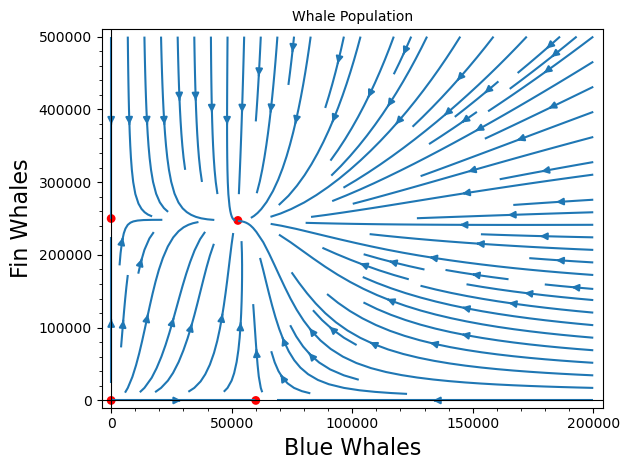
\includegraphics[width=0.65\linewidth]{images/ex3vectorfield.png}
    \caption{Vector field for Exercise 3, part (a) in Chapter 5 with equilibriums in red.}
\end{figure}

\begin{table}[h!]
    \centering
    \begin{tabular}{llllll}
        \toprule
        \textbf{Blue Whales} & \textbf{Fin Whales} & \textbf{Eigen 1} & \textbf{Eigen 2} & \textbf{Type} & \textbf{Stability} \\\midrule
        \(0\) & \(0\) & \(0.020\) & \(0.051\) & Source & Unstable\\
        \(60000\) & \(0\) & \(0.051\) & \(-0.020\) & Saddle & Unstable\\
        \(0\) & \(250000\) & \(0.018\) & \(-0.051\) & Saddle & Unstable\\
        \(52579\) & \(247371\) & \(-0.051\) & \(-0.020\) & Sink & Stable\\
        \bottomrule
    \end{tabular}
    \caption{Each equilibrium's location in \hyperref[fig:ex3pta]{Figure 1} with type and stability specified.}\label{tab:ex3pta}
\end{table}

\begin{enumerate}
    \setcounter{enumi}{2}
    \item Reconsider Exercise 6 of Chapter 4. Assume that the catchability coefficient \(q = 10^{-5}\) and that the level of effort is \(E = 3000\) boat-days per year.
    \begin{enumerate}
        \item  Sketch the vector field for this model. Determine the location of each equilibrium in the state space.
        \sol{
            \hyperref[fig:ex3pta]{Figure 1} gives us the vector field for this model. \hyperref[tab:ex3pta]{Table 1} gives each location of each equilibrium.
        }
        \item Use the eigenvalue method to test the stability of each equilibrium in the state space.
        \sol{
            \hyperref[tab:ex3pta]{Table 1} gives the stability of each equilibrium.
        }
    \end{enumerate}
\newpage
\begin{figure}[h!]
    \label{fig:ex3ptc}
    \centering
    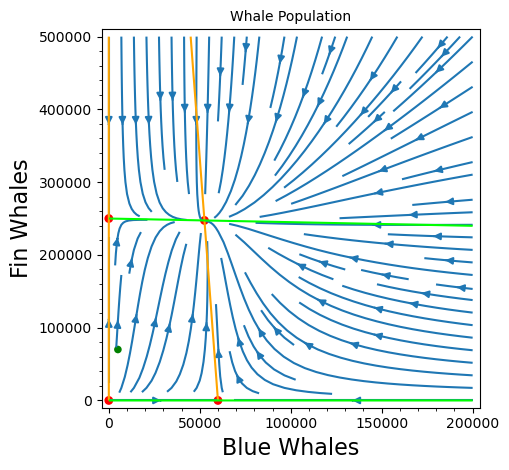
\includegraphics[width=0.45\linewidth]{images/ex3pportrait.png}
    \caption{Phase portrait for Exercise 3, part (c) in Chapter 5 with \(x\)-nullclines in green, and \(y\)-nullclines in orange. The green dot is added to visualize the population for part (d).}
\end{figure}

    \begin{enumerate}
        \setcounter{enumii}{3}
        \item  Sketch the complete phase portrait for this model, using the results of parts (a) and (c).
        \sol{
            Phase portrait pictured in \hyperref[fig:ex3ptc]{Figure 2}.
        }
        \item Given the current estimates of 5000 blue whales and 70,000 fin whales, what does this model predict about the future of the two species?
        \sol{
            The model predicts that the two species will survive. By following the streamplot in \hyperref[fig:ex3ptc]{Figure 2}, we can see that both species will trend toward the stable equilibrium at \((52579, 247371)\).
        }
    \end{enumerate}
\end{enumerate}

\begin{figure}[h!]
    \label{fig:ex4pta}
    \centering
    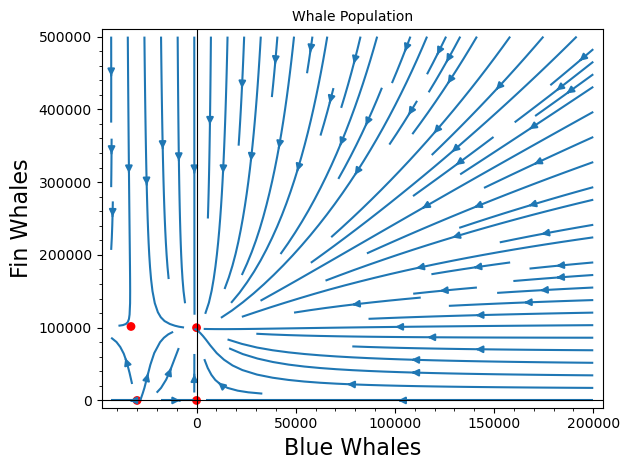
\includegraphics[width=0.55\linewidth]{images/ex4vectorfield.png}
    \caption{Vector field for Exercise 4, part (a) in Chapter 5 with equilibriums in red.}
\end{figure}

\newpage

\begin{table}[t]
    \centering
    \begin{tabular}{llllll}
        \toprule
        \textbf{Blue Whales} & \textbf{Fin Whales} & \textbf{Eigen 1} & \textbf{Eigen 2} & \textbf{Type} & \textbf{Stability} \\\midrule
        \(0\) & \(0\) & \(-0.0098\) & \(0.020\) & Saddle & Unstable \\
        \(-30000\) & \(0\) & \(0.020\) & \(0.0098\) & Source & Unstable \\
        \(0\) & \(100000\) & \(-0.011\) & \(-0.020\) & Sink & Stable \\
        \(-33050\) & \(101652\) & \(-0.020\) & \(0.011\) & Saddle & Unstable\\
        \bottomrule
    \end{tabular}
    \caption{Each equilibrium's location in \hyperref[fig:ex4pta]{Figure 3} with type and stability specified.}\label{tab:ex4pta}
\end{table}

\begin{enumerate}
    \setcounter{enumi}{3}
    \item Repeat Exercise 3, but now assume a level of effort of \(E = 6000\) boat-days per year.
    \begin{enumerate}
        \item  Sketch the vector field for this model. Determine the location of each equilibrium in the state space.
        \sol{
            \hyperref[fig:ex4pta]{Figure 3} gives us the vector field for this model. \hyperref[tab:ex4pta]{Table 2} gives each location of each equilibrium.
        }
        \item Use the eigenvalue method to test the stability of each equilibrium in the state space.
        \sol{
            \hyperref[tab:ex4pta]{Table 2} gives the stability of each equilibrium.
        }
        \setcounter{enumii}{3}
        \item  Sketch the complete phase portrait for this model, using the results of parts (a) and (c).
        \sol{
            Phase portrait pictured in \hyperref[fig:ex4ptc]{Figure 4}.
        }
        \item Given the current estimates of 5000 blue whales and 70,000 fin whales, what does this model predict about the future of the two species? 
        \sol{
            The model predicts that blue whales will quickly go extinct. It also predicts that the fin whales will reach a stable equilibrium at \((0, 100000)\).
        }
    \end{enumerate}
\end{enumerate}

\begin{figure}[h!]
    \label{fig:ex4ptc}
    \centering
    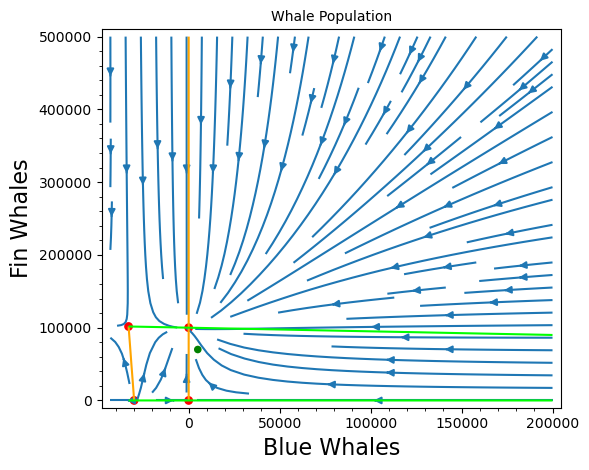
\includegraphics[width=0.40\linewidth]{images/ex4pportrait.png}
    \caption{Phase portrait for Exercise 4, part (c) in Chapter 5 with \(x\)-nullclines in green, and \(y\)-nullclines in orange. The green dot is added to visualize the population for part (d).}
\end{figure}


\newpage

\section*{Chapter 6}

\begin{table}[h!]
    \centering
    \begin{tabular}{llll}
        \toprule
        \(w\) & \textbf{Winner} & \textbf{Remaining} & \textbf{Time (days)} \\\midrule
        \(0.2\) & Red & \(2.07\) & \(48.9\) \\
        \(0.5\) & Red & \(2.8\) & \(19.5\) \\
        \(0.75\) & Red & \(3.03\) & \(13.0\) \\
        \(0.9\) & Red & \(3.11\) & \(10.9\) \\
        \bottomrule
    \end{tabular}
    \caption{Simulation results for varying values of \(w\) with \(\lambda = 3\) in Eq. 6.20.}\label{tab:ex1ptb}
\end{table}

\begin{enumerate}
    \item Reconsider the war problem of Example 6.1. In this problem we explore the effects of weather on combat. Bad weather and poor visibility decrease the effectiveness of direct fire weapons for both sides. The effectiveness of indirect fire weapons is relatively unaffected by the weather. We can represent the effects of bad weather in our model as follows. Let \(w\) denote the decrease in weapon effectiveness caused by bad weather conditions, and replace the dynamical system in Eq. (6.3) by
    \begin{align*}
        \Delta x_{1} &= -w\lambda(0.05) x_{2} - \lambda (0.005)x_{1}x_{2} \\
        \Delta x_{2} &= -w0.05 x_{1} - 0.005x_{1}x_{2}
    \end{align*}
    \begin{enumerate}
        \item Use a computer implementation of the algorithm in Fig. 6.2 to simulate the discrete–time dynamical system in Eq. (6.20) in the case \(\lambda = 3\). Assume that adverse weather conditions cause a 75\% decrease in weapon effectiveness for both sides (\(w = 0.25\)). Who wins the battle, and how long does it take? How many divisions of troops remain on the winning side?
        \sol{
            With the given parameters of \(\lambda = 3\) and \(w = 0.25\), the simulation returns that Red wins the battle, they have 2.28 divisions remaining, and the battle lasted 39.0 days. 
        }
        \item Repeat your analysis for each of the cases \(w = 0.1\), 0.2, 0.5, 0.75, and 0.9, and tabulate your results. Answer the same questions as in part (a).
        \sol{
            The tabulated results are presented in \hyperref[tab:ex1ptb]{Table 3}. In the table, we can see that as \(w\) increases, so does red's efficiency. In fact, for \(w = 0.9\), red almost quintuples their time efficiency, and an additional division survives in comparison to \(w = 0.2\). 
        }
        \item Which side benefits from fighting in adverse weather conditions? If you were the blue commander, would you expect red to attack on a sunny day or a rainy day?
        \sol{
            It appears that red gains a significant advantage from poor weather. The blue commander should expect an attack on a rainy day.
        }
    \end{enumerate}
\end{enumerate}

\newpage

\begin{figure}[h!]
    \label{fig:ex8pta}
    \centering
    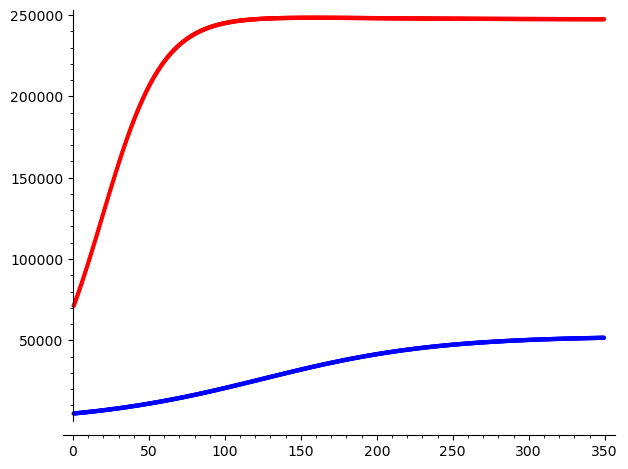
\includegraphics[width=0.50\linewidth]{images/ex8bluefinvstime.png}
    \caption{Blue whales (blue line) and fin whales (red line) plotted over time for Exercise 8, part (a) in Chapter 6.}
\end{figure}


\begin{enumerate}
    \setcounter{enumi}{7}
    \item Reconsider Exercise 6 in Chapter 4, and assume \(\alpha = 10^{-8}\). Assume that the current population levels are \(B = 5\),000 and \(F = 70\),000.
    \begin{enumerate}
        \item Use a computer implementation of the simple algorithm used in Section 6.2 to determine the effect of harvesting. Assume \(E =\) 3,000 boat–days per year. What happens to the two species of  whales over the long term, according to this model? Do both species of whales grow back, or will one or both species become extinct? How long does this take?
        \sol{
            Given a harvesting rate of \(E = 3000\) boat-days per year and a starting population of 5,000 and 70,000 for blue and fin whales respectively, we can expect both whales will grow back. They will reach a stable equilibrium around the population of \((52579, 247371)\). However, it will take approximately 349.5 years to reach these levels. We also notice in \hyperref[fig:ex8pta]{Figure 5} that the fin whales grow back much quicker than the blue whale.
        }
        \setcounter{enumii}{3}
        \item Repeat part (c) for the specific cases \(\alpha = 10^{-9}\), \(10^{-8}\), \(10^{-6}\), and \(10^{-5}\), and tabulate your results. Discuss the sensitivity of your conclusions to the extent of interspecies competition.
        \sol{
            From \hyperref[tab:ex8ptd]{Table 4}, we can see that there is a general trend: As we increase \(E\), the upper bound for both whale populations decreases. Then, for \(\alpha = 10^{-6}\) and \(10^{-5}\), we also see that the fin whales consistently break out the blue whales, but the competition does not affect the upper limit for the whale populations. In general, we see that an increase in the competition factor leads to the extinction of blue whales. For the entries with times exceeding 1,000 years, further analysis shows that the fin whales live, but the blue whales are going extinct very slowly.  
        }
    \end{enumerate}
\end{enumerate}

\begin{table}[t]
    \centering
    \begin{tabular}{lllll}
        \toprule
        \textbf{Blue Whales} & \textbf{Fin Whales} & \textbf{Time (years)} & \(\alpha\) & \(E\) \\\midrule
        \(117970\) & \(349415\) & \(199\) & \(10^{-9}\) & \(1000\) \\
        \(108665\) & \(344618\) & \(209\) & \(10^{-8}\) & \(1000\) \\
        \(0\) & \(350000\) & \(10000\) & \(10^{-6}\) & \(1000\) \\
        \(0\) & \(209890\) & \(27.0\) & \(10^{-5}\) & \(1000\) \\
        \(88112\) & \(299564\) & \(245.50\) & \(10^{-9}\) & \(2000\) \\
        \(80126\) & \(296032\) & \(260\) & \(10^{-8}\) & \(2000\) \\
        \(0\) & \(300000\) & \(10000\) & \(10^{-6}\) & \(2000\) \\
        \(0\) & \(205809\) & \(34.5\) & \(10^{-5}\) & \(2000\) \\
        \(58255\) & \(249712\) & \(326\) & \(10^{-9}\) & \(3000\) \\
        \(51579\) & \(247447\) & \(349.50\) & \(10^{-8}\) & \(3000\) \\
        \(0\) & \(250000\) & \(10000\) & \(10^{-6}\) & \(3000\) \\
        \(0\) & \(203739\) & \(50.5\) & \(10^{-5}\) & \(3000\) \\
        \(28404\) & \(199859\) & \(502.50\) & \(10^{-9}\) & \(4000\) \\
        \(23039\) & \(198860\) & \(550.50\) & \(10^{-8}\) & \(4000\) \\
        \(0\) & \(200000\) & \(10000\) & \(10^{-6}\) & \(4000\) \\
        \(0\) & \(200000\) & \(10000\) & \(10^{-5}\) & \(4000\) \\
        \(550\) & \(149997\) & \(3412.5\) & \(10^{-9}\) & \(5000\) \\
        \(0\) & \(150000\) & \(10000\) & \(10^{-8}\) & \(5000\) \\
        \(0\) & \(150000\) & \(10000\) & \(10^{-6}\) & \(5000\) \\
        \(0\) & \(150000\) & \(10000\) & \(10^{-5}\) & \(5000\) \\
        \bottomrule
    \end{tabular}
    \caption{Blue and fin whales competition with competition coefficient, \(\alpha\), and effect of harvesting, \(E\) for Exercise 8, part (d) in Chapter 6.}\label{tab:ex8ptd}
\end{table}

\end{document}